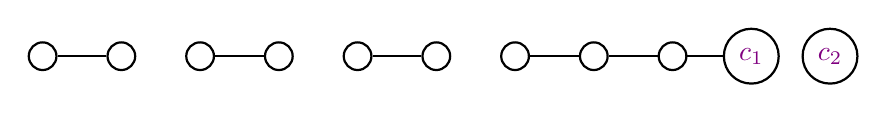
\begin{tikzpicture}[auto, thick]
\tikzstyle{vertex}=[draw,circle,text=violet,minimum width=10pt]
  \foreach \place/\name in {{(0,0)/a},
                            {(1,0)/b},
                            {(2,0)/c},
                            {(3,0)/d},
                            {(4,0)/e},
                            {(5,0)/f},
                            {(6,0)/g},
                            {(7,0)/h},
                            {(8,0)/i}}
    \node[vertex] (\name) at \place {};
  \node[vertex] (j) at (9,0) {$c_1$};
  \node[vertex] (k) at (10,0) {$c_2$};
  \foreach \source/\dest in {a/b,c/d,e/f,g/h,h/i,i/j}
      \path (\source) edge (\dest);
\end{tikzpicture}